\chapter{関連研究}
\makeendnotes  %フットノートをすべて章末に移動するスクリプトです。使用しない場合はコメントアウトしてください。

\section{フラッシュマーケティングについて}
\subsection{フラッシュマーケティングとは}
フラッシュマーケティングとはインターネットを使って、商品やサービス利用料をクーポンとして割り引き販売する手法のことである。“フラッシュが光るような短期間”で販売し終えることからちなんで名づけられた。そのため販売時間は24時間~48時間という短時間がほとんどで、この間に出品者が設定した数量が売り切れれば取引が成立し、予定数の注文に達しなければ販売は成立しないというシステムになっている。
また宣伝効果も期待でき、話題性のある商品を出品することで、SNSといった口コミを誘いやすく、宣伝効果は高い。専用サイトでは、取引成立までの残時間をカウントダウン表示することで、購買意欲を高めるなどの工夫があるのが特徴だ。

具体的に従来のクーポンサイトとの違いは矢内で以下5つが挙げられている。
\begin{enumerate}
	\item \textbf{消費の前にチケットを購入する必要がある}
	\\事前購入という方法は、消費者にとっては負担が大きいが、店舗の視点から考えれば売り上げが見込め、従来の街角で配布しているクーポンに比べ、広告費の削減につながる。
	\item \textbf{購入のための期間が限定されている}
	\\期間が限定されていることで、消費者の注目を集める大きな要素となっており、消費者の決断を迫るリアクタンス理論 (Brehm, 1966; Brehm  Brehm,1981) を用いた効率的な販売手法である。
	\item\textbf{取引成立の最少人数が決まっている}
	\\最少人数を設定することで、人数に達しなければ成立しないので、成立させたいという思いから友人や他社をSNS等々でクーポンの情報を拡散させる。実際に2012年8月21日~9月20日の31日間に行われた398件の取引の分析結果を見ると10件しか不成立に終わっていない \cite{yauchi}
	また米国GROUPONの購読者調査によると66%がGROUPONの記事を見ている。結果として魅力的なクーポンが出された場合には即座に成立することになる。
	\\店舗側からすると削減される費用を割引として還元することで、他のクーポンよりも思い切った値段設定ができるという仕組みである。
	\item \textbf{割引率が高いものが多く、50%を超えるものが一般的}
	\\フラッシュマーケティングサイトの一番の特徴ともいえるのが価格の割引率である。新規開店やリニューアル、低稼働時など様々なシーンでクーポンを出して集客を図るのがフラッシュマーケティングの一般的な使い方である。
	\\先述した期間限定の特徴とも相まって消費者の意識をひきつけ購買へ結びついてると考えられる。
	\item \textbf{特定の業種に限った紹介ではなく、一般的には1day 1area 1deal 形式で様々な形式が紹介される}
	\\ぐるなびや一休のような従来のインターネット経由のクーポンの提供方法は、特定の業種に絞ってクーポンが提供されることが通例であった。これではユーザーは特定のサービスが必要な時にだけサイトに接触することになりユーザーとの接点は途切れがちになる。
	\\上記のサイトに比較してフラッシュマーケティングサイトは様々なクーポンを提供できるのだが、1day 1area 1dealという形式をとっている。これは従来のあふれんばかりの情報を整理し、消費者の居住地や趣味嗜好を基にシンプルな提案を行うことで購買活動を促している。
\end{enumerate}

\subsection{フラッシュマーケティングサイトのビジネスモデル}
上述のように、クーポン購入者を時間限定でサイト上で募集し、申し込みが規定数を超えれば割引された特別価格でのクーポンの発行が成立する。売り上げの 20〜50%は手数料として共同購入サイトに払われ、残りは店舗側の利益として支払われる。結果、クーポン購入者へは店舗側からサービスが提供される。
\\
\begin{figure}[htbp]
	\centering
	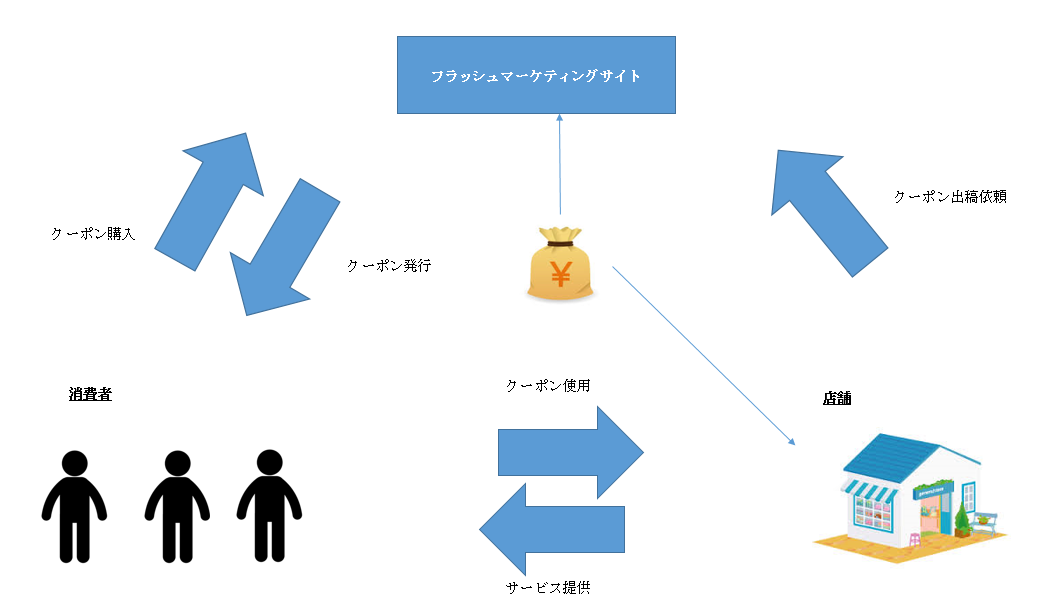
\includegraphics[width=6cm, bb=0 0 640 480]{figures/soukin.jpg}
	\caption{ビジネスモデル}
	\label{ビジネスモデル}
\end{figure}
\\
\\
店舗側からすれば客の入りが少ない時間帯を格安で提供することで、消費者を呼ぶことができ、新規顧客の獲得につながる。
\subsection{フラッシュマーケティングサイトの販売手法の転換}

次にフラッシュマーケティングの歴史について紹介する。フラッシュマーケティングの歴史は共同購入にあるといわれている。共同購入とは国内では生協のかつての販売スタイルに起因する。生協の組合員が一週間以上前に注文した商品が、翌週に班やグループに配達される仕組みのことを指す。(川口、毛利、和歌森、2005) 複数人で一つの商品を購入することで送料を下げることができ安価に購入できるというメリットがあった。1970年代にはこの無店舗事業で生協は首都圏で大きく売り上げ伸ばしていった。
\\ しかしこの生協のモデルは後に誰がどの様な商品を、購入しているのかわかってしまう、近所付き合い上やめにくくなってしまうなど人間関係上多くのデメリットがあり、人々は個人の宅に配送する宅配コープデリ (個送) を選択するようになる。
\\
\\
\begin{figure}[htbp]
	\centering
	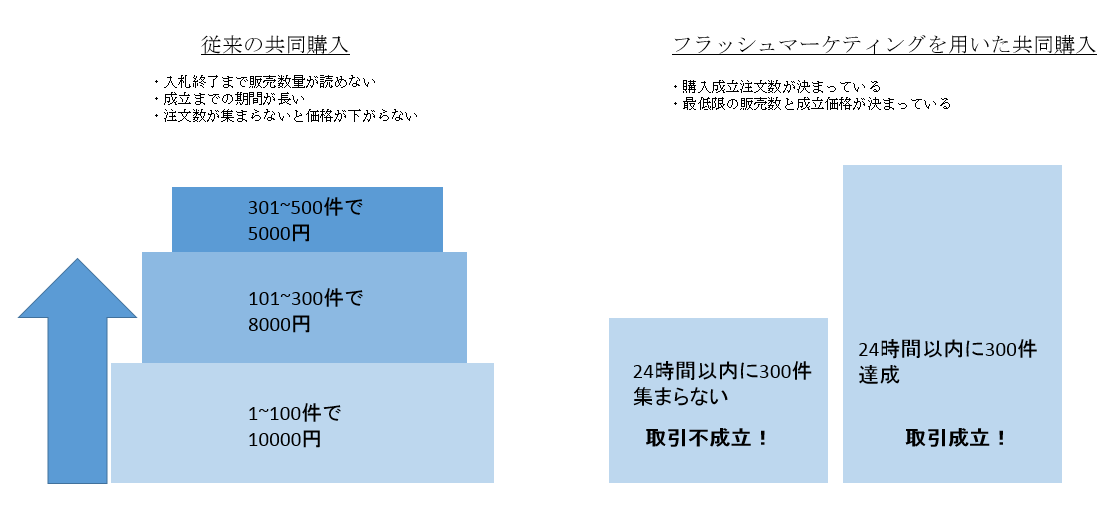
\includegraphics[width=85mm, bb=0 0 600 272]{figures/fm.jpg}
	\caption{フラッシュマーケティング市場推移 {\itshape coupon-jp.com}}
	\label{フラッシュマーケティング市場推移}
\end{figure}
\\2000年にはいるとインターネットが普及し始め、インターネット上で共同購入サイトが勃興し始めた。当初は左図のような仕組みで共同購入がの仕組みがとられていた。時間内に共同購入者を募れば募るほど、商品を割引されていくことがメリットであった。しかし以下2点の問題があった。(日経ビジネス、「話題のフラッシュマーケティングの全てがわかる」)
\begin{itemize}
	\item 注文数が集まらないと価格が下がらない
	\item 入札までの販売数がわからない
\end{itemize}

従来の共同購入では、利用者側からすると、購入した後に自身の希望する金額に減額するまでは、共同購入者を募らなければならず、最終的な購買価格もましてや購入できるのかどうかさえわからない。従来の共同購入は入札期間が1週間以上あるので、利用者は購入を先延ばしにする傾向にあり、店舗側と共同購入サイトは機会損失を生みやすかった。
\\ フラッシュマーケティングを用いり、最低成立人数を決めることで、一定の人数を集めることで、商品を購入でき、最低限の販売数も読めるようになり近年の見られるように売上が上昇した。

\subsection{フラッシュマーケティングの現状}
日本では2010年4月にサービス開始したグルーポンをはじめ、ポンパレがシェアを占めている。大手企業も参入し、リクルートのポンパレ、楽天グループのRaCoupon「買うクーポン」などがある。2010年6月時点では6社参入であったが、2010年10月時点で100サイトを超え、2011年12月時点では230サイトを超えている
日本国内におけるフラッシュマーケティングの市場推移はほぼ横ばい状態で月の売り上げは30億円程度で推移している。毎年多く企業がフラッシュマーケティング市場に参入するがグルーポンとポンパレで市場の8割ほどを占めている。
\\
\begin{figure}[htbp]
	\centering
	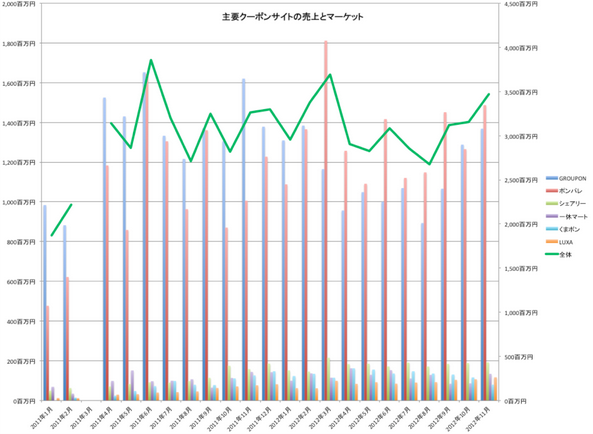
\includegraphics[width=6cm, bb=0 0 330 272]{figures/shijo.jpg}
	\caption{フラッシュマーケティング市場推移 {\itshape coupon-jp.com}}
	\label{フラッシュマーケティング市場推移}
\end{figure}
\newpage
日本国内の売上をカテゴリー別で売上を見ると、飲食の売上が圧倒的に占めている。さらに日本国内の割合とアメリカのフラッシュマーケティング市場の代替指標としてのグルーポンUS、中国のフラッシュマーケティング市場の代替指標としての中国の主要サービス10社の売上をカテゴリー別に比較した。ここでも飲食の割合が大きいのは元々、食べログやホットペッパーといった飲食におけるクーポンサイトが存在し、消費者にとって飲食分野における教育コストが低かったことが考えられる。
\begin{figure}[htbp]
	\centering
	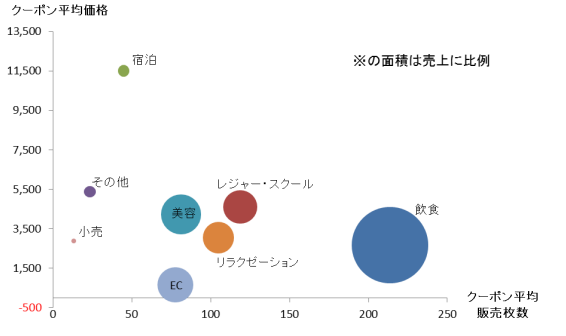
\includegraphics[width=6cm, bb=0 0 330 272]{figures/cate.jpg}
	\caption{各カテゴリー別売上 {\itshape yauchi,2012}}
	\label{各カテゴリー別売上}
\end{figure}
\begin{figure}[htbp]
	\centering
	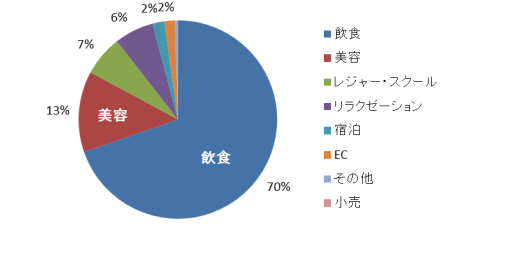
\includegraphics[width=6cm, bb=0 0 330 272]{figures/gjp.jpg}
	\caption{国内フラッシュマーケティングの売上割合 {\itshape http://ipfm.jp/dl/101224FlashMarketingFreeVER1-1.pdf}}
	\label{国内フラッシュマーケティングの売上割合}
	\end{figure}
	
\begin{figure}[htbp]
	\centering
	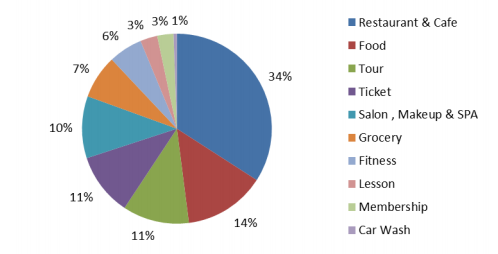
\includegraphics[width=6cm, bb=0 0 330 272]{figures/gus.jpg}
	\caption{グルーポンのアメリカにおけるカテゴリー別売上 {\itshape coupon-jp.com}}
	\label{グルーポンのアメリカにおけるカテゴリー別売上}
\end{figure}

\begin{figure}[htbp]
	\centering
	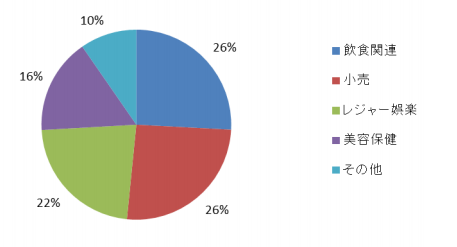
\includegraphics[width=6cm, bb=0 0 330 272]{figures/gc.jpg}
	\caption{中国におけるにおけるフラッシュマーケティング市場のカテゴリー別売上 {\itshape coupon-jp.com}}
	\label{中国におけるにおけるフラッシュマーケティング市場のカテゴリー別売上}
\end{figure}
\section{各サイトの特徴}
この節では国内の代表的なフラッシュマーケティングサイトを紹介する。
\subsection{Gropon}
Grouponは、アメリカ合衆国イリノイ州シカゴに本社を置き、共同購入型クーポンサイト「Groupon」を運営する米国の企業である。2008年10月にシカゴのピザ半額キャンペーンから始まった。日本国内では2010年6月にサービスを開始し、現在では国内の売上シェア1位である。
\\顧客獲得方法は、友人を紹介した利用者に対し、1000円程度のサイト内で使えるクーポンを配布したことで、顧客を増やしてきた。
\\国内でシェアを獲得できた理由は、従来の後払い時にクーポンを提示する従来のクーポンに対し、Grouponは前払い決済でサービスを受けられるので、クーポン発行後の損失がなく、大幅値引きが可能で利用率も高くなった。飲食、美容系(ヘアサロン、ネイルサロンなど)など後払いなので、クーポンを多数発券しても利用率は低くかったが、Grouponが前払いを採用し、利用率は上昇し、効果の見えるプロモーションが可能になったと言われている。
\subsection{ポンパレ}
ポンパレは全国に幅広い営業拠点をもつ株式会社リクルートライフスタイルが提供するフラッシュマーケティングサイトである。同業界では後発のサービスであるが、他社とは対照的にレジャー・スクールのクーポンの割合が多く、国内の市場では売上シェアが2位である。
対応エリアは東京、大阪などの主要都市から始まり、2010年11月現在ではほぼ全国をカバーしている。また、リクルートが提供する「じゃらん」「ケイコとマナブ」などのサービスとの連携も特徴となっている。

\section{フットサルのマッチングサービス}
\subsection{footlink}
footlink(フットリンク)は、フットサルやサッカー(ソサイチ)の対戦相手募集中チームを検索し、試合を申し込むサイトである。利用者はまずメールアドレスで登録し、ログインしたとに、対戦したい相手を図の画面から選択する。
\\
\\
\\
\\
\begin{figure}[htbp]
	\centering
	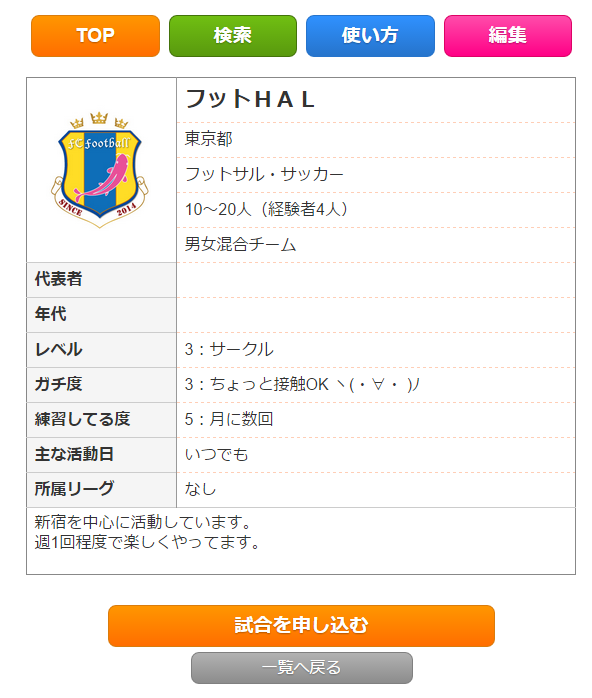
\includegraphics[width=85mm, bb=0 0 800 272]{figures/fl.jpg}
	\caption{footlinkにおける試合相手選択画面 {\itshape http://footlink.net/}}
	\label{footlinkにおける試合相手選択画面}
\end{figure}
\\
\\
選択した後、相手チームから返信がくれば試合を組めることになり、両者で試合の日時、場所を専用取引フォームで進めていくこととなる。
\\ 原則として対戦チーム数は2チームで催され、どちらかがフットサルコートの会員でないとサービスは進行できない。

\subsection{EnjoyFutsal}
EnjoyFutsalはフットボールスマイル株式会社が運営するフットサルチーム同士のマッチングサービスである。メールアドレスで新規登録した後に、画面の図から試合を募集しているチームを選択することで、試合を組むことができる。
\begin{figure}[htbp]
	\centering
	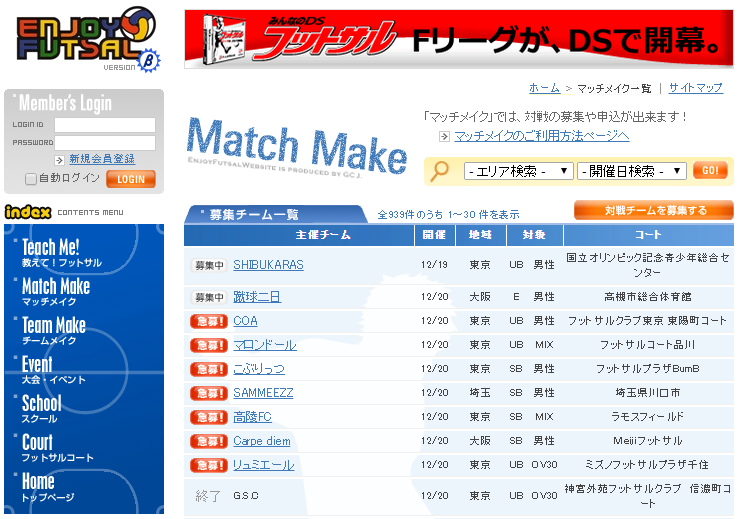
\includegraphics[width=85mm, bb=0 0 800 272]{figures/ef.jpg}
	\caption{EnjoyFutsalにおける試合相手選択画面 {\itshape enjoyfutsal.com}}
	\label{EnjoyFutsalにおける試合相手選択画面}
\end{figure}
\\
\\
\\
\\
特徴としては、3チーム以上のマッチングができる点とチームメイクができる点が、FootLinkと異なる。
\\ 画面にあるように募集チームは男女別、さらにはポジション別にメンバーを募集できる。
\\
\\
\\
\\
\\
\\
\begin{figure}[htbp]
	\centering
	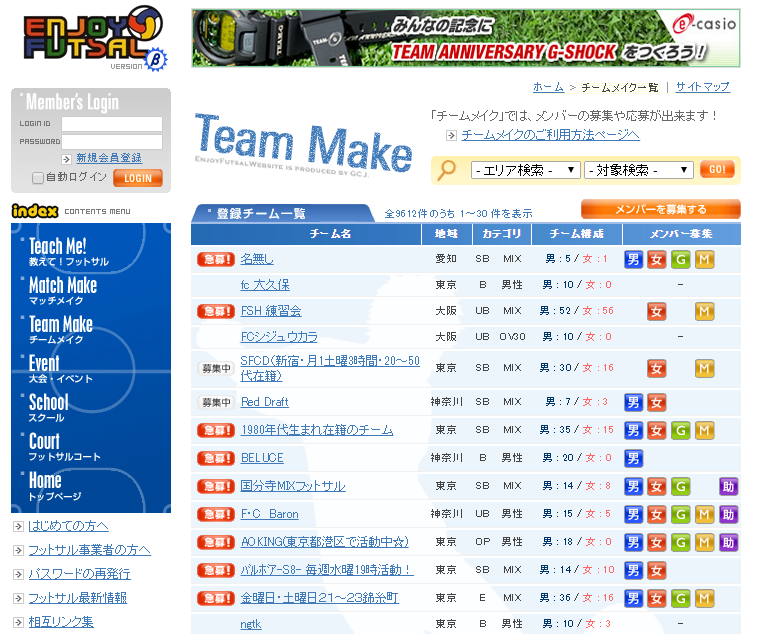
\includegraphics[width=85mm, bb=0 0 800 272]{figures/mm.jpg}
	\caption{footlinkにおける試合相手選択画面 {\itshape enjoyfutsal.com}}
	\label{EnjoyFutsalにおける部員募集画面}
\end{figure}
\section{フラッシュマーケティングの有効性}
フラッシュマーケティングには、クーポンとしての経済的効果と共同購入としての経済学的効果があるとで述べられている。
\subsection{クーポンの経済学的効果}
まずクーポンについての経済学的効果として(玉井、2010)では出稿する店舗側には広告効果、価格差別、スイッチングコスト、リピート効果の4つが述べられている。
本サービスでは、価格とリピート効果に関連し、サービスを構築したのでここでは価格とリピート効果についてどのような経済的効果があるのか述べる。
\subsubsection{価格差別}
クーポン戦略の2つ目の利点は価格差別が行ることである。価格差別には以下3点の特徴がある。 (西岡、2010)
\begin{itemize}
	\item 第1価格差別
	\\財の売り手が、「買い手が支払ってもいい最大の金額」を完全に把握していて、かつ買い手ごとに異なる価格を提示できる。
	\item 第2価格差別
	\\財の売り手は、買い手の特徴や購買意欲によっては異なる価格を提示できないが、財の個数(や品質)と価格の組み合わせを非線形にして提示できる。
	\\具体例としてはガス料金や電気料金といった公共料金、携帯電話の使用料金が挙げられる。
	\item 第3価格差別
	\\財の売り手は、買い手の購買意欲によって異なる価格を提示することはできないが、買い手の特徴(性別、年齢、地域など)によって異なる価格を提示できる。
	\\具体的な例としては,学生割引,女性割引,子供料金,シニアー料金が挙げられる。	
\end{itemize}
Webにおけるクーポンは消費者の登録情報を基に効率よく提供されているので、第3種価格差別が当てはまるので、ここでは第3種価格差別の話を進めていく。
\subsubsection{リピート効果}
\subsection{共同購入の経済学的効果}
(Evan Miller,2012) によると図で多数の購買者が集まって低価格で買うことにコミットすれば従来にない需要と供給のマッチングポイントが生まれ、買い手と売り手にっとって新しい有効性があると論じている。
\begin{figure}[htbp]
	\centering
	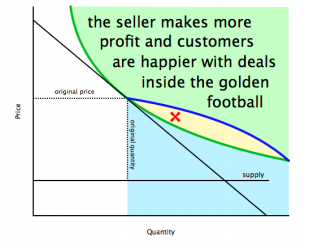
\includegraphics[width=85mm, bb=0 0 200 272]{figures/nush.jpg}
	\caption{フラッシュマーケティングにおける価格均衡点 {\itshape http://www.evanmiller.org/golden-football.html}}
	\label{フラッシュマーケティングにおける価格均衡点}
\end{figure}
